\section*{\MakeUppercase{Appendices}}
\addcontentsline{toc}{section}{\MakeUppercase{Appendices}}

\appendix

% Appendix sections must be numbered as letters: A, B, C, and so on.
\renewcommand{\thesubsection}{\Alph{subsection}}

\subsection{Some First Title}\label{apx:A}

And here is an example of a footnote made in the Appendix section.\footnote{This is another example of a footnote, which is in Appendix~\ref {apx:A}.}

\subsubsection*{Some title}
\lipsum[1]

\subsubsection*{Some title}
\lipsum[2]

\begin{figure}[!ht]
    \vspace{.4in}
    % The figure's caption and notes lines are centered, 100% of page width 
    \captionsetup{width=1\linewidth,labelfont=bf}
    \caption{Example of a plot, showing daily data on interest rates in the U.S, from Appendix~\ref{apx:A}}
    \vspace{.2in}
    \centering
    % The plot is 100% of its width
    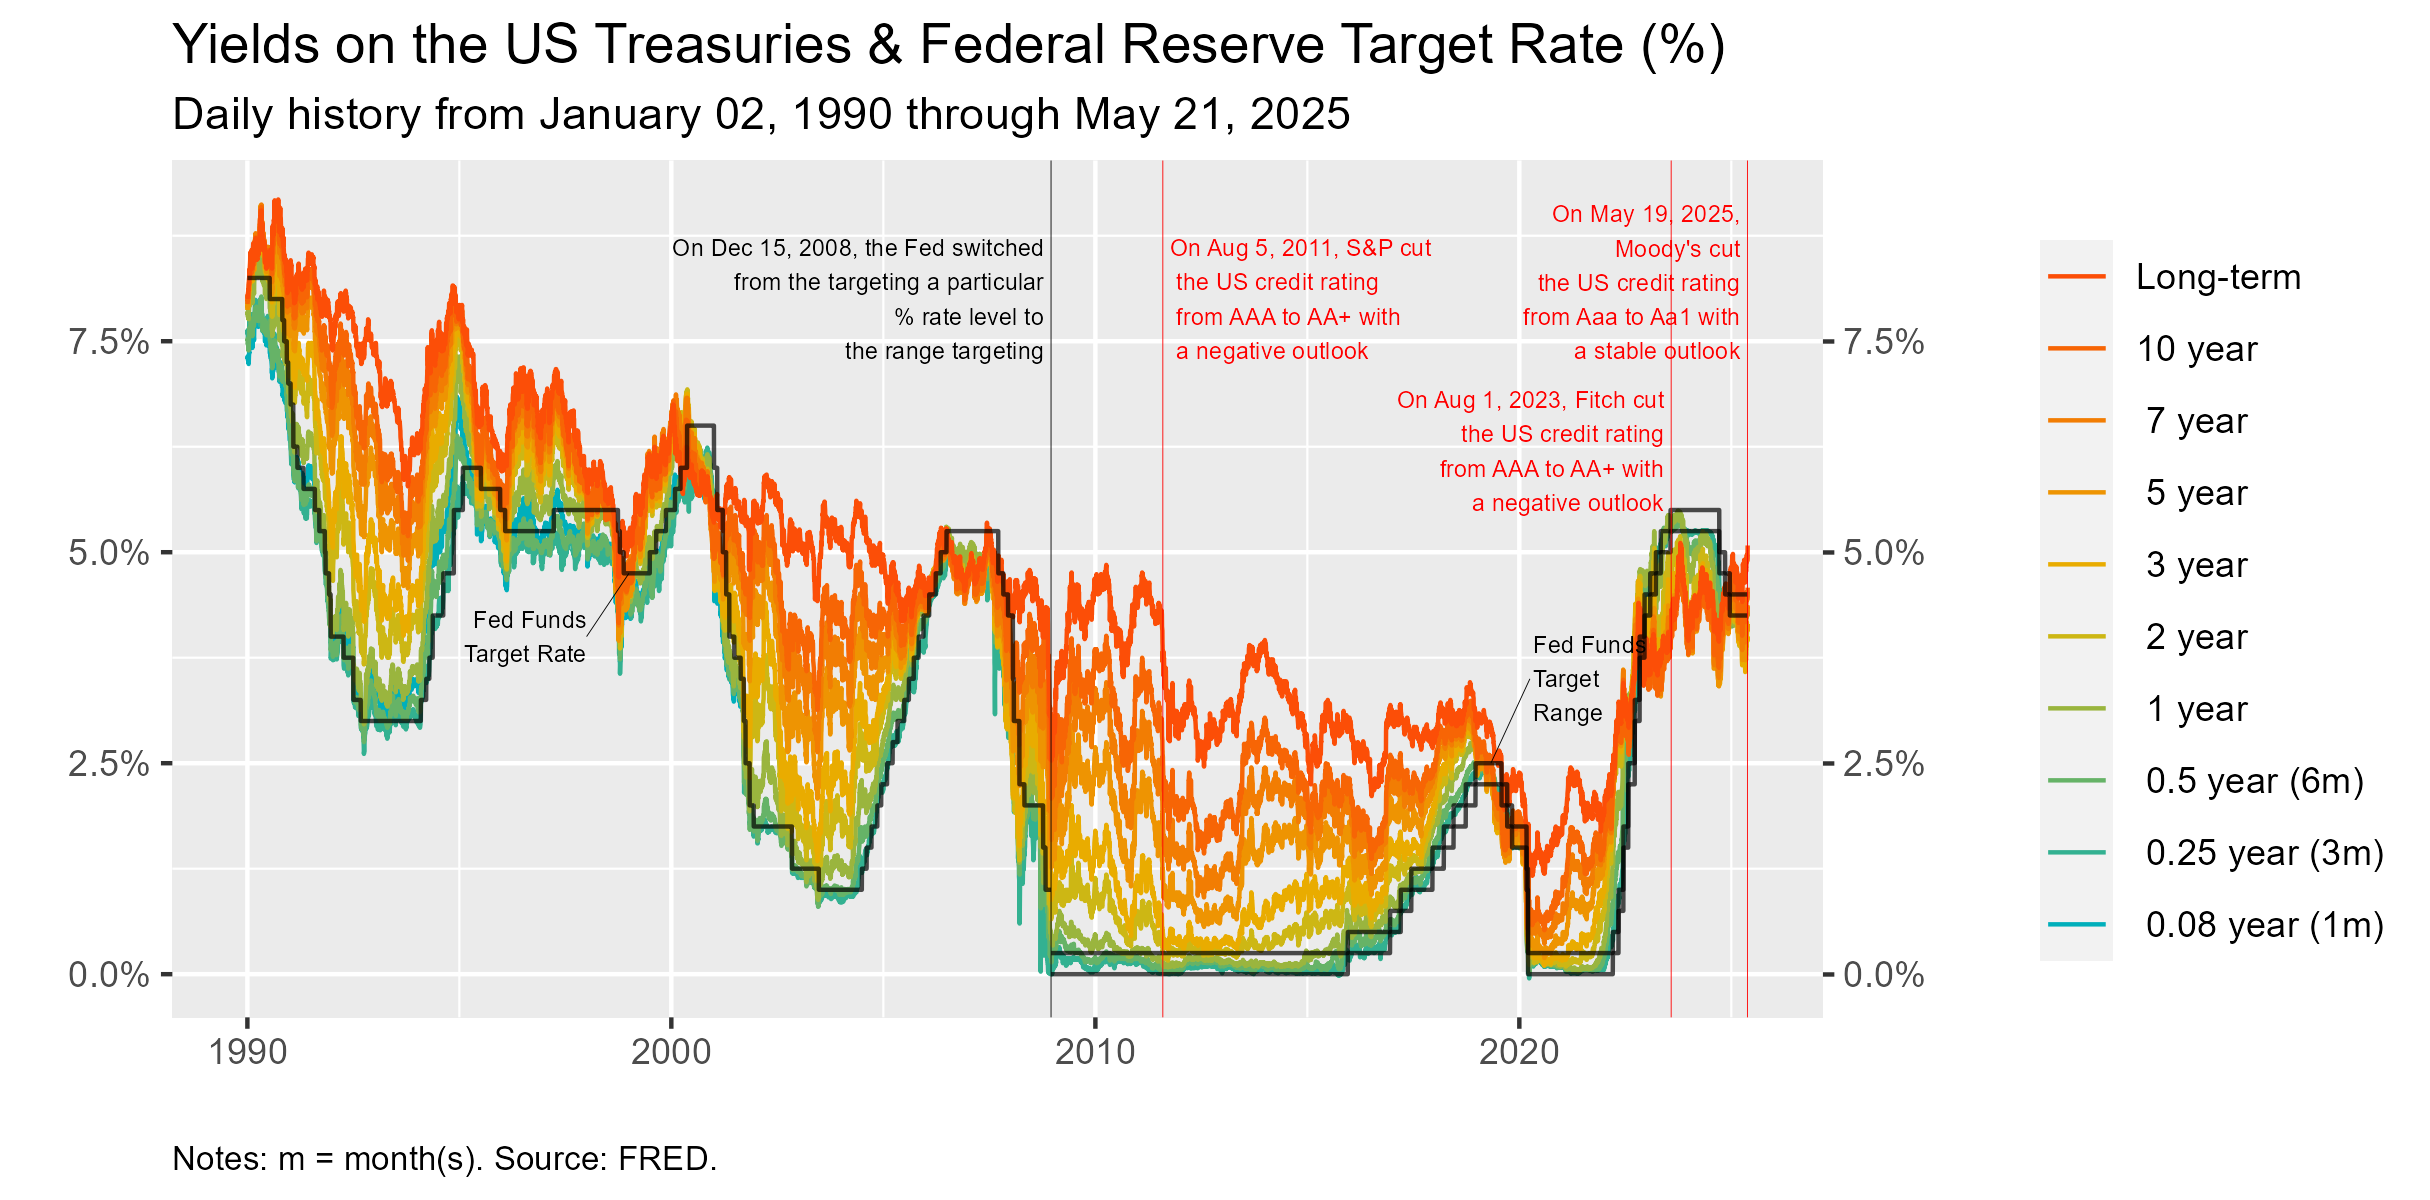
\includegraphics[width=1\linewidth]{Plots/Plot 3.png}
    \vspace{.2in}
    \caption*{Note: some notes. \par\vspace{.15in} Source: Federal Reserve System of the United States}
    \vspace{.2in}
    \label{fig:plot3}
\end{figure}

\lipsum[3]

\subsection{Some Second Title}\label{apx:B}

\subsubsection*{Some title}
\lipsum[4]

\begin{figure}[htbp]
    \vspace{.2in}
    % The figure's caption and notes lines are centered, 100% of page width 
    \captionsetup{width=1\linewidth,labelfont=bf}
    \caption{Example of a large plot, showing monthly data points, which is placed on a separate page in Appendix~\ref{apx:B}}
    \vspace{.2in}
    \centering
    % The plot is 100% of its width
    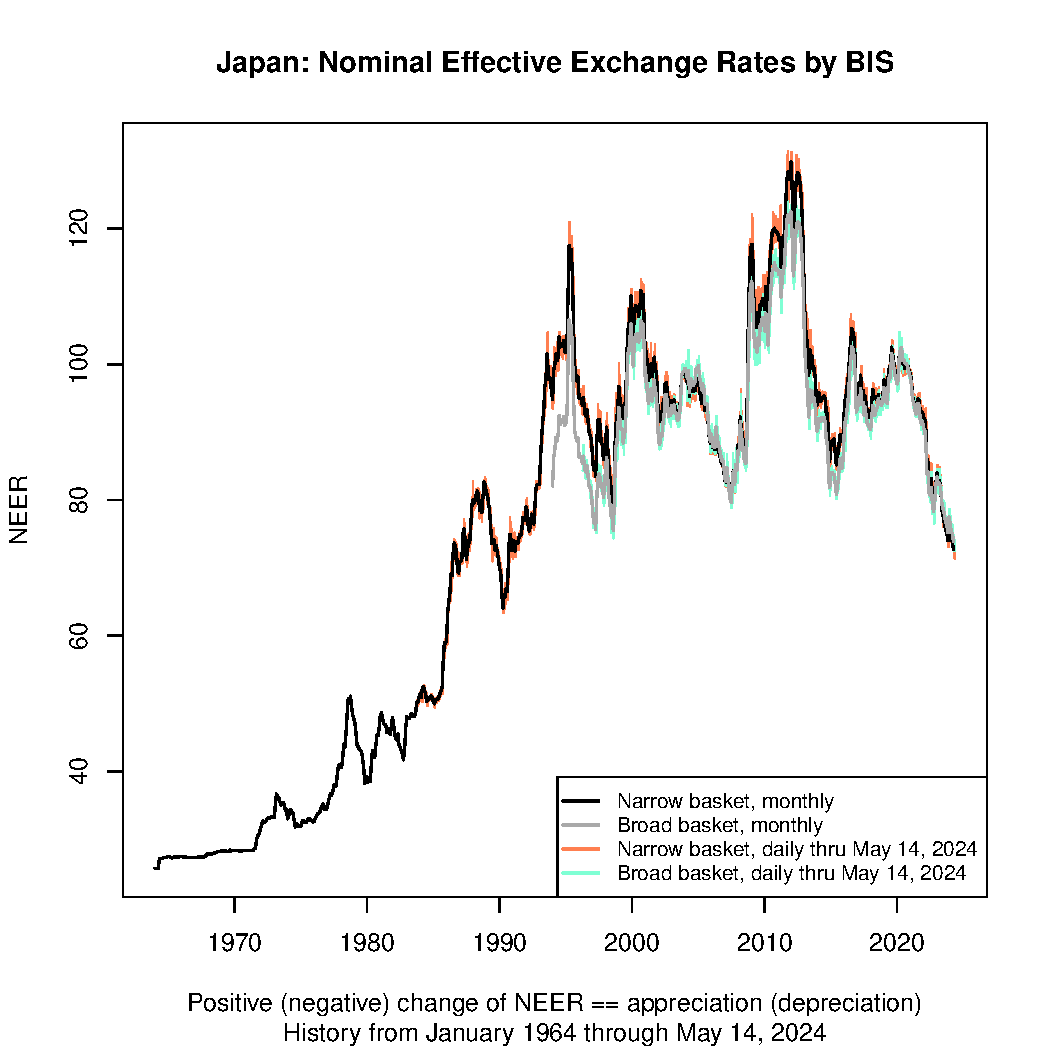
\includegraphics[width=1\linewidth]{Plots/Plot 2.pdf}
    \vspace{.2in}
    \caption*{Note: some notes. \par\vspace{.15in} Source: \ac{bis}, \url{https://www.bis.org/}}
    \vspace{.2in}
    \label{fig:plot2}
\end{figure}

\subsubsection*{Some title}
\lipsum[5]

\begin{sidewaysfigure}[htbp]
    \captionsetup{width=1\linewidth,labelfont=bf}
    \caption{Example of an elaborate, landscape \emph{TiKz} plot}
    \begin{tikzpicture}[scale=.85]
    \draw[help lines,white] (0,0) grid (26,14);
    \draw[black,dashed] (8.5,-1) -- (8.5,14.25); 
    \draw[black,dashed] (17.5,-1) -- (17.5,14.25); 
    \node[red]  at (4.5,14) {\textsuperscript{\MakeUppercase{Great Britain} (British pound \pounds, GBP)}};
    \node[blue] at (13,14) {\textsuperscript{\MakeUppercase{United States} (U.S. dollar \$, USD)}};
    \node[purple] at (22,14) {\textsuperscript{\MakeUppercase{Poland} (Polish zloty, PLN)}};
  % US ====================================================
    % NY Fed ------------------------------------------------------------
        \node [matrix,fill=gray!10,draw=black,thin,font=\bf\fontsize{8}{8}\selectfont] (cb) at (11,11) {
            \node {Assets}; & \node {Liab's}; \\
            \node (CB_c0) {$c_0$}; & \node[rectangle,draw=blue,thick] (CB_d0)  {$\overrightarrow{d}_0$}; \\
            \node {$c_t$}; & \node {$d_t$}; \\
            \node {$\widetilde{c}$}; & \node {$\widetilde{d}$}; \\
            };
        \draw (cb)++(0,1.5) node[font=\bf\fontsize{7}{7}\selectfont]%
            {New York Fed $CB_2$};
    % Bank R1 ------------------------------------------------------------
        \node [matrix,fill=gray!10,draw=black,thin,font=\bf\fontsize{8}{8}\selectfont] (cb) at (11,7) {
            \node {Assets}; & \node {Liab's}; \\
            \node[rectangle,draw=blue,thick] (R1_c0) {$\overrightarrow{c}_0$}; & \node[rectangle,draw=blue,thick] (R1_d0) {$\overrightarrow{d}_0$}; \\
            \node {$c_t$}; & \node {$d_t$}; \\
            \node {$\widetilde{c}$}; & \node {$\widetilde{d}$}; \\
            };
        \draw (cb)++(0,1.5) node[font=\bf\fontsize{7}{7}\selectfont]%
            {Bank $R_2$};
    % Clearing Authority -------------------------------------------------
        \node [matrix,fill=gray!10,draw=black,thin,font=\bf\fontsize{8}{8}\selectfont] (CA2) at (15,7) {
            \node {Assets}; & \node {Liab's}; \\
            \node[rectangle,draw=blue,thick] (CA2_c0) {$\overrightarrow{c}_0$}; & \node[rectangle,draw=blue,thick] (CA2_d0) {$\overrightarrow{d}_0$}; \\
            \node {$c_t$}; & \node {$d_t$}; \\
            \node {$\widetilde{c}$}; & \node {$\widetilde{d}$}; \\
            \node {}; & \node {}; \\
            \node[rectangle,draw=red,thick] (CA2_fx1_c0) {$\overrightarrow{c}_0$}; & \node (CA2_fx_d0) {$d_0$}; \\
            \node {$c_t$}; & \node {$d_t$}; \\
            \node {$\widetilde{c}$}; & \node {$\widetilde{d}$}; \\
            \node {}; & \node {}; \\
            \node[rectangle,draw=purple,thick] (CA2_fx3_c0) {$\overrightarrow{c}_0$}; & \node (CA2_fx_d0) {$d_0$}; \\
            \node {$c_t$}; & \node {$d_t$}; \\
            \node {$\widetilde{c}$}; & \node {$\widetilde{d}$}; \\
            };
        \draw[dashed] (CA2.west)++(0,.75) -- +(2.8,0) node[at end ,right,font=\fontsize{8}{8}\selectfont] {\$/\pounds};
        \draw[dashed] (CA2.west)++(0,-1.2) -- +(2.8,0) node[at end ,right,font=\fontsize{8}{8}\selectfont] {\$/zloty};
        \draw (CA2)++(0,3.8) node[font=\bf\fontsize{7}{7}\selectfont]%
            {Clearing Auth. $CA_2$};
    % Exporter ----------------------------------------------
        \node [matrix,fill=gray!10,draw=black,thin,font=\bf\fontsize{8}{8}\selectfont] (cb) at (11,3) {
            \node {Assets}; & \node {Liab's}; \\
            \node[rectangle,draw=blue,thick] (B_c0) {$\overrightarrow{c}_0$}; & \node {$d_0$}; \\
            \node {$c_t$}; & \node {$d_t$}; \\
            \node {$\widetilde{c}$}; & \node {$\widetilde{d}$}; \\
            };
        \draw (cb)++(0,1.5) node[font=\bf\fontsize{7}{7}\selectfont]%
            {Exporter Firm $B$};
    \gettikzxy{(CB_d0)}{\ax}{\ay}; \gettikzxy{(R1_c0)}{\bx}{\by}
    \draw[blue] (CB_d0.east) -- (13,11.2) -- (13,9) -- (9,9) -- (9,\by) -- (R1_c0.west);
    \gettikzxy{(CB_d0)}{\ax}{\ay}; \gettikzxy{(CA2_c0)}{\bx}{\by}
    \draw[blue] (CB_d0.east) -- (13.2,\ay) -- (13.2,\by) -- (CA2_c0.west);
    \gettikzxy{(R1_d0)}{\ax}{\ay}; \gettikzxy{(B_c0)}{\bx}{\by}
    \draw[blue] (R1_d0.east) -- (13,\ay) -- (13,5) -- (9,5) -- (9,\by) -- (B_c0.west);
    \draw[blue,thick] (10,-.5) node(a)[draw] {} (11,-.5) node(b)[draw] {};
    \draw[blue,thick] (a) -- (b);
    \node[black,align=left,font=\fontsize{8}{8}\selectfont] at (13.8,-.5)%
        {DCR due today continuously\\and denominated in U.S. dollar};
    % MX ====================================================
    % BoE ----------------------------------------------------------
        \node [matrix,fill=gray!10,draw=black,thin,font=\bf\fontsize{8}{8}\selectfont] (cb) at (2,11) {
            \node {Assets}; & \node {Liab's}; \\
            \node (CB_c0) {$c_0$}; & \node[rectangle,draw=red,thick] (CB_d0)  {$\overrightarrow{d}_0$}; \\
            \node {$c_t$}; & \node {$d_t$}; \\
            \node {$\widetilde{c}$}; & \node {$\widetilde{d}$}; \\
            };
        \draw (cb)++(0,1.5) node[font=\bf\fontsize{7}{7}\selectfont]%
            {Bank of England $CB_1$};
    % Bank R2 ------------------------------------------------------------
        \node [matrix,fill=gray!10,draw=black,thin,font=\bf\fontsize{8}{8}\selectfont] (cb) at (2,7) {
            \node {Assets}; & \node {Liab's}; \\
            \node[rectangle,draw=red,thick] (R2_c0) {$\overrightarrow{c}_0$}; & \node[rectangle,draw=red,thick] (R2_d0) {$\overrightarrow{d}_0$}; \\
            \node {$c_t$}; & \node {$d_t$}; \\
            \node {$\widetilde{c}$}; & \node {$\widetilde{d}$}; \\
            };
        \draw (cb)++(0,1.5) node[font=\bf\fontsize{7}{7}\selectfont]%
            {Bank $R_1$};
    % Clearing Authority -------------------------------------------------
        \node [matrix,fill=gray!10,draw=black,thin,font=\bf\fontsize{8}{8}\selectfont] (CA1) at (6,7) {
            \node {Assets}; & \node {Liab's}; \\
            \node[rectangle,draw=red,thick] (CA1_c0) {$\overrightarrow{c}_0$}; & \node[rectangle,draw=red,thick] (CA1_d0) {$\overrightarrow{d}_0$}; \\
            \node {$c_t$}; & \node {$d_t$}; \\
            \node {$\widetilde{c}$}; & \node {$\widetilde{d}$}; \\
            \node {}; & \node {}; \\
            \node[rectangle,draw=blue,thick] (CA1_fx2_c0) {$\overrightarrow{c}_0$}; & \node (CA1_fx_d0) {$d_0$}; \\
            \node {$c_t$}; & \node {$d_t$}; \\
            \node {$\widetilde{c}$}; & \node {$\widetilde{d}$}; \\
            \node {}; & \node {}; \\
            \node[rectangle,draw=purple,thick] (CA1_fx3_c0) {$\overrightarrow{c}_0$}; & \node (CA1_fx_d0) {$d_0$}; \\
            \node {$c_t$}; & \node {$d_t$}; \\
            \node {$\widetilde{c}$}; & \node {$\widetilde{d}$}; \\
            };
        \draw[dashed] (CA1.west)++(0,.75) -- +(2.8,0) node[at end ,right,font=\fontsize{8}{8}\selectfont] {\pounds/\$};
        \draw[dashed] (CA1.west)++(0,-1.2) -- +(2.8,0) node[at end ,right,font=\fontsize{8}{8}\selectfont] {\pounds/zloty};
        \draw (CA1)++(0,3.8) node[font=\bf\fontsize{7}{7}\selectfont]%
            {Clearing Auth. $CA_1$};
    % Exporter ----------------------------------------------
        \node [matrix,fill=gray!10,draw=black,thin,font=\bf\fontsize{8}{8}\selectfont] (cb) at (2,3) {
            \node {Assets}; & \node {Liab's}; \\
            \node[rectangle,draw=red,thick] (A_c0) {$\overrightarrow{c}_0$}; & \node {$d_0$}; \\
            \node {$c_t$}; & \node {$d_t$}; \\
            \node {$\widetilde{c}$}; & \node {$\widetilde{d}$}; \\
            };
        \draw (cb)++(0,1.5) node[font=\bf\fontsize{7}{7}\selectfont]%
            {Importer Firm $A$};
    \gettikzxy{(CB_d0)}{\ax}{\ay}; \gettikzxy{(R2_c0)}{\bx}{\by}
    \draw[red] (CB_d0.east) -- (4,11.2) -- (4,9) -- (0,9) -- (0,\by) -- (R2_c0.west);
    \gettikzxy{(CB_d0)}{\ax}{\ay}; \gettikzxy{(CA1_c0)}{\bx}{\by}
    \draw[red] (CB_d0.east) -- (4.2,\ay) -- (4.2,\by) -- (CA1_c0.west);
    \gettikzxy{(R2_d0)}{\ax}{\ay}; \gettikzxy{(A_c0)}{\bx}{\by}
    \draw[red] (R2_d0.east) -- (4,\ay) -- (4,5) -- (0,5) -- (0,\by) -- (A_c0.west);
    \draw[red,thick] (1,-.5) node(a)[draw] {} (2,-.5) node(b)[draw] {};
    \draw[red,thick] (a) -- (b);
    \node[black,align=left,font=\fontsize{8}{8}\selectfont] at (5,-.5)%
        {DCR due today continuously\\and denominated in British pound};
    % PL ====================================================
    % Bank of Poland ----------------------------------------------------------
        \node [matrix,fill=gray!10,draw=black,thin,font=\bf\fontsize{8}{8}\selectfont] (cb) at (20,11) {
            \node {Assets}; & \node {Liab's}; \\
            \node (CB_c0) {$c_0$}; & \node[rectangle,draw=purple,thick] (CB_d0)  {$\overrightarrow{d}_0$}; \\
            \node {$c_t$}; & \node {$d_t$}; \\
            \node {$\widetilde{c}$}; & \node {$\widetilde{d}$}; \\
            };
        \draw (cb)++(0,1.5) node[font=\bf\fontsize{7}{7}\selectfont]%
            {Narodowy Bank Polski $CB$};
    % Bank R3 ------------------------------------------------------------
        \node [matrix,fill=gray!10,draw=black,thin,font=\bf\fontsize{8}{8}\selectfont] (cb) at (20,7) {
            \node {Assets}; & \node {Liab's}; \\
            \node[rectangle,draw=purple,thick] (R2_c0) {$\overrightarrow{c}_0$}; & \node[rectangle,draw=purple,thick] (R2_d0) {$\overrightarrow{d}_0$}; \\
            \node {$c_t$}; & \node {$d_t$}; \\
            \node {$\widetilde{c}$}; & \node {$\widetilde{d}$}; \\
            };
        \draw (cb)++(0,1.5) node[font=\bf\fontsize{7}{7}\selectfont]%
            {Bank $R_3$};
    % Clearing Authority -------------------------------------------------
        \node [matrix,fill=gray!10,draw=black,thin,font=\bf\fontsize{8}{8}\selectfont] (CA3) at (24,7) {
            \node {Assets}; & \node {Liab's}; \\
            \node[rectangle,draw=purple,thick] (CA3_c0) {$\overrightarrow{c}_0$}; & \node[rectangle,draw=purple,thick] (CA3_d0) {$\overrightarrow{d}_0$}; \\
            \node {$c_t$}; & \node {$d_t$}; \\
            \node {$\widetilde{c}$}; & \node {$\widetilde{d}$}; \\
            \node {}; & \node {}; \\
            \node[rectangle,draw=blue,thick] (CA3_fx2_c0) {$\overrightarrow{c}_0$}; & \node (CA3_fx_d0) {$d_0$}; \\
            \node {$c_t$}; & \node {$d_t$}; \\
            \node {$\widetilde{c}$}; & \node {$\widetilde{d}$}; \\
            \node {}; & \node {}; \\
            \node[rectangle,draw=red,thick] (CA3_fx1_c0) {$\overrightarrow{c}_0$}; & \node (CA3_fx_d0) {$d_0$}; \\
            \node {$c_t$}; & \node {$d_t$}; \\
            \node {$\widetilde{c}$}; & \node {$\widetilde{d}$}; \\
            };
        \draw[dashed] (CA3.west)++(0,.75) -- +(2.8,0) node[at end ,right,font=\fontsize{8}{8}\selectfont] {zloty/\$};
        \draw[dashed] (CA3.west)++(0,-1.2) -- +(2.8,0) node[at end ,right,font=\fontsize{8}{8}\selectfont] {zloty/\pounds};
        \draw (CA3)++(0,3.8) node[font=\bf\fontsize{7}{7}\selectfont]%
            {Clearing Auth. $CA_3$};
    % Exporter ----------------------------------------------
        \node [matrix,fill=gray!10,draw=black,thin,font=\bf\fontsize{8}{8}\selectfont] (cb) at (20,3) {
            \node {Assets}; & \node {Liab's}; \\
            \node[rectangle,draw=purple,thick] (A_c0) {$\overrightarrow{c}_0$}; & \node {$d_0$}; \\
            \node {$c_t$}; & \node {$d_t$}; \\
            \node {$\widetilde{c}$}; & \node {$\widetilde{d}$}; \\
            };
        \draw (cb)++(0,1.5) node[font=\bf\fontsize{7}{7}\selectfont]%
            {Importer Firm $C$};
    \gettikzxy{(CB_d0)}{\ax}{\ay}; \gettikzxy{(R2_c0)}{\bx}{\by}
    \draw[purple] (CB_d0.east) -- (22,11.2) -- (22,9) -- (18,9) -- (18,\by) -- (R2_c0.west);
    \gettikzxy{(CB_d0)}{\ax}{\ay}; \gettikzxy{(CA3_c0)}{\bx}{\by}
    \draw[purple] (CB_d0.east) -- (22.2,\ay) -- (22.2,\by) -- (CA3_c0.west);
    \gettikzxy{(R2_d0)}{\ax}{\ay}; \gettikzxy{(A_c0)}{\bx}{\by}
    \draw[purple] (R2_d0.east) -- (22,\ay) -- (22,5) -- (18,5) -- (18,\by) -- (A_c0.west);
    \draw[purple,thick] (19,-.5) node(a)[draw] {} (20,-.5) node(b)[draw] {};
    \draw[purple,thick] (a) -- (b);
    \node[black,align=left,font=\fontsize{8}{8}\selectfont] at (23,-.5)%
        {DCR due today continuously\\and denominated in Polish zloty};
    % ================================================================
    \gettikzxy{(CA1_fx3_c0)}{\ax}{\ay}; \gettikzxy{(CA3_d0)}{\bx}{\by}
    \draw[purple] (CA1_fx3_c0.west) -- (4.4,\ay) -- (4.4,.6) -- (26,.6) -- (26,\by) -- (CA3_d0.east);
    \gettikzxy{(CA2_fx3_c0)}{\ax}{\ay}; \gettikzxy{(CA3_d0)}{\bx}{\by}
    \draw[purple] (CA2_fx3_c0.west) -- (13.2,\ay) -- (13.2,.8) -- (25.8,.8) -- (25.8,9.1) -- (CA3_d0.east);
    \gettikzxy{(CA1_fx2_c0)}{\ax}{\ay}; \gettikzxy{(CA2_d0)}{\bx}{\by}
    \draw[blue] (CA1_fx2_c0.west) -- (4.2,\ay) -- (4.2,.4) -- (17,.4) -- (17,9.1) -- (CA2_d0.east);
    \gettikzxy{(CA3_fx2_c0)}{\ax}{\ay}; \gettikzxy{(CA2_d0)}{\bx}{\by}
    \draw[blue] (CA3_fx2_c0.west) -- (22.4,\ay) -- (22.4,.4) -- (17.2,.4) -- (17.2,\by) -- (CA2_d0.east);
    \gettikzxy{(CA3_fx1_c0)}{\ax}{\ay}; \gettikzxy{(CA1_d0)}{\bx}{\by}
    \draw[red] (CA3_fx1_c0.west) -- (22.2,\ay) -- (22.2,1) -- (8,1) -- (8,9.1) -- (CA1_d0.east);
    \gettikzxy{(CA2_fx1_c0)}{\ax}{\ay}; \gettikzxy{(CA1_d0)}{\bx}{\by}
    \draw[red] (CA2_fx1_c0.west) -- (13.4,\ay) -- (13.4,1.2) -- (8.2,1.2) -- (8.2,\by) -- (CA1_d0.east);
\end{tikzpicture}

    \caption*{Notes: some notes here. \par\vspace{.15in} Source: \url{https://github.com/valchyshen}}
    \label{fig:tikz2}
\end{sidewaysfigure}